%%%%%%%%%%%%%%%%%%%%%%%%%%%%%%%%%%%%%%%%%%%%%%%%%%%%%%%%%%%%%%%%%%%%%%%%%%%%%%%%%%%%
% Document data
%%%%%%%%%%%%%%%%%%%%%%%%%%%%%%%%%%%%%%%%%%%%%%%%%%%%%%%%%%%%%%%%%%%%%%%%%%%%%%%%%%%%
\documentclass[12pt]{article} %report allows for chapters
%%%%%%%%%%%%%%%%%%%%%%%%%%%%%%%%%%%%%%%%%%%%%%%%%%%%%%%%%%%%%%%%%%%%%%%%%%%%%%%%%%%%
\usepackage{preamble}

\begin{document}

\begin{center}
   \textsc{\large MATH 271, Homework 7, \emph{Solutions}}\\
   \textsc{Due November 1$^\textrm{st}$}
\end{center}
\vspace{.5cm}

\begin{problem}
Let $S$ be the set of general solutions $x(t)$ to the following homogeneous linear differential equation 
\[
x''+f(t)x'+g(t)x=0.
\]
Show that this set $S$ is a vector space over the complex numbers by doing the following. Let $x(t),y(t) \in S$ be solutions to the above equation and let $\alpha, \beta \in \C$ be complex scalars.
\begin{enumerate}[(a)]
    \item Write down the eight requirements for $S$ to be a vector space.  
    \item Identify the $\zerovec \in S$ and $1\in \C$. 
    \item Show that $\alpha x(t) + \beta y(t) \in S$. That is, show that a superposition of solutions is also a solution. \emph{Hint: We have shown this before.}
\end{enumerate}
\end{problem}
\begin{solution}
\begin{enumerate}[(a)]
    \item We can remember these requirements via the acronym CANI ADDU.  So we have for the vector addition properties
    \begin{itemize}
        \item Commutivity: If we have two solutions $x(t)$ and $y(t)$ in the set $S$, then we know 
        \[
        x(t)+y(t)=y(t)+x(t)
        \]
        is satisfied.
        \item Associativity: If we have three solutions $x(t),y(t),z(t)\in S$, then we know
        \[
        (x(t)+y(t))+z(t)=x(t) + (y(t)+z(t))
        \]
        is satisfied.
        \item Neutral Element: We have that there exists the zero function $0\in S$ such that
        \[
        0+x(t)=x(t).
        \]
        \item Inverses: Given an $x(t)\in S$, we have the function $-x(t)\in S$ such that
        \[
        x(t)+(-x(t))=0.
        \]
    \end{itemize}
    Then we have the scalar multiplication properties
    \begin{itemize}
        \item Associativity: If we have $\alpha,\beta \in \C$ and $x(t)\in S$ then we have
        \[
        \alpha (\beta x(t)) = (\alpha \beta)x(t)
        \]
        holds.
        \item Distribution: Given $\alpha,\beta \in \C$ and $x(t)\in S$ we have
        \[
        (\alpha +\beta)x(t) = \alpha x(t) + \beta x(t)
        \]
        holds.
        \item Distribution: Given $\alpha\in \C$ and $x(t),y(t)\in S$, we have
        \[
        \alpha(x(t)+y(t))=\alpha x(t) + \alpha y(t)
        \]
        holds.
        \item Unit element: We have $1\in \C$ satisfies that for any $x(t)\in S$ that
        \[
        1 x(t) = x(t).
        \]
    \end{itemize}
    \item Now, note that above we defined $\zerovec\in S$ to be the zero function 0. That is, the function that is 0 for every value of $t$. Note that $0$ is a solution to the equation since
    \[
    0'' + f(t)\cdot 0' + g(t) 0 = 0.
    \]
    Then, we have $1\in \C$ that satisfies the necessary property to. In this case, 1 is literally the unit element we care about.  
    
    \begin{remark} 
        Not all vector spaces will have such obvious neutral elements, $\zerovec$, or unit elements $1$.  This is why we must be a bit careful at times.
    \end{remark}
    \item Now, the biggest requirement for a vector space is that linear combinations of vectors actually produce another vector. This is quite obvious in the plane $\R^2$ for example, but here, it is not necessarily obvious.  
    
    Now, we take $\alpha,\beta \in \C$ and $x(t),y(t)\in S$ and we consider the linear combination
    \[
    z(t) = \alpha x(t) + \beta y(t).
    \]
    We then wish to show that this linear combination (or superposition) is a solution as well. So we plug in $z(t)$ into our equation as follows
    \begin{align*}
        z''(t)+f(t)z'(t)+g(t)z(t)&= (\alpha x''(t) + \beta y''(t))+f(t)(\alpha x'(t) + \beta y'(t))+g(t)(\alpha x(t)+\beta y(t))\\
        &= \alpha \left[x''(t)+f(t)x'(t)+g(t)x(t)\right] + \beta \left[ y''(t)+f(t)y'(t)+g(t)y(t)\right]\\
        &=0,
    \end{align*}
    since we knew that $x(t)$ and $y(t)$ themselves are solutions. Thus, $z(t)$ is as well and now we have that $S$ is a vector space.
\end{enumerate}
\end{solution}

\newpage
\begin{problem}
Consider the following vectors in the real plane $\R^2$. We let
\[
\vecu = 1\xhat + 2\yhat \qquad \textrm{and} \qquad \vecv = -3\xhat+ 3\yhat.
\]
\begin{enumerate}[(a)]
    \item Draw both $\vecu$ and $\vecv$ in the plane and label the origin.
    \item Draw the vector $\vecw = \vecu+\vecv$ in the plane.
    \item Find the area of the parallelogram generated by $\vecu$ and $\vecv$.
\end{enumerate}
\end{problem}
\begin{solution}
\begin{enumerate}[(a)]
    \item See the plane below.
    \item Both (a) and (b) are in the plane here:
    \begin{center}
        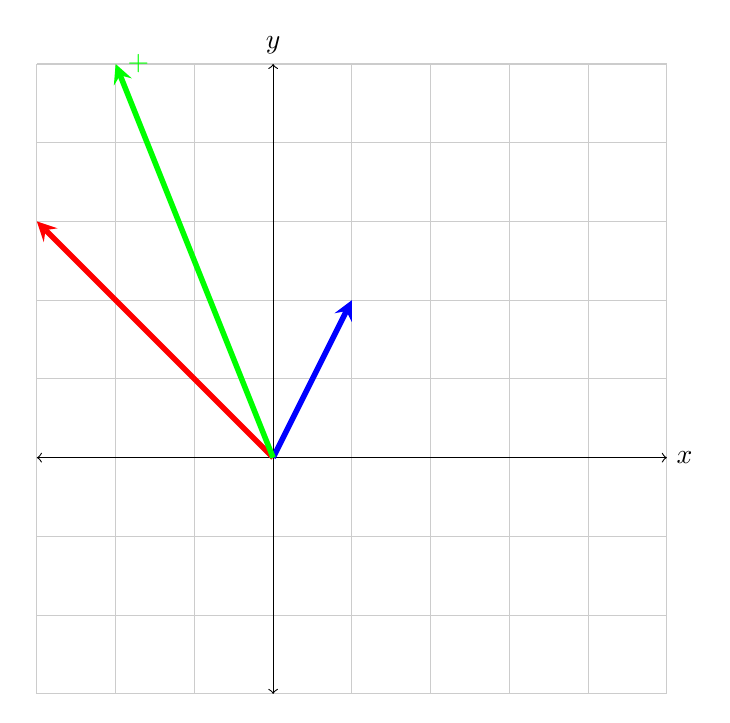
\begin{tikzpicture}
        \draw[thin,gray!40] (-3,-3) grid (5,5);
        \draw[<->] (-3,0)--(5,0) node[right]{$x$};
        \draw[<->] (0,-3)--(0,5) node[above]{$y$};
        \draw[line width=2pt,blue,-stealth](0,0)--(1,2) node[anchor=west] at (1,2){$\vecu$};
        \draw[line width=2pt, red, -stealth](0,0)--(-3,3) node[anchor=north] at (-3,3){$\vecv$};
        \draw[line width=2pt, green, -stealth](0,0)--(-2,5) node[anchor=west] at (-2,5){$\vecu+\vecv$};
        \end{tikzpicture}
        \end{center}
        \item One could compute the area of the parallelogram generated by $\vecu$ and $\vecv$ in many ways. First, let us see what this looks like:
            \begin{center}
        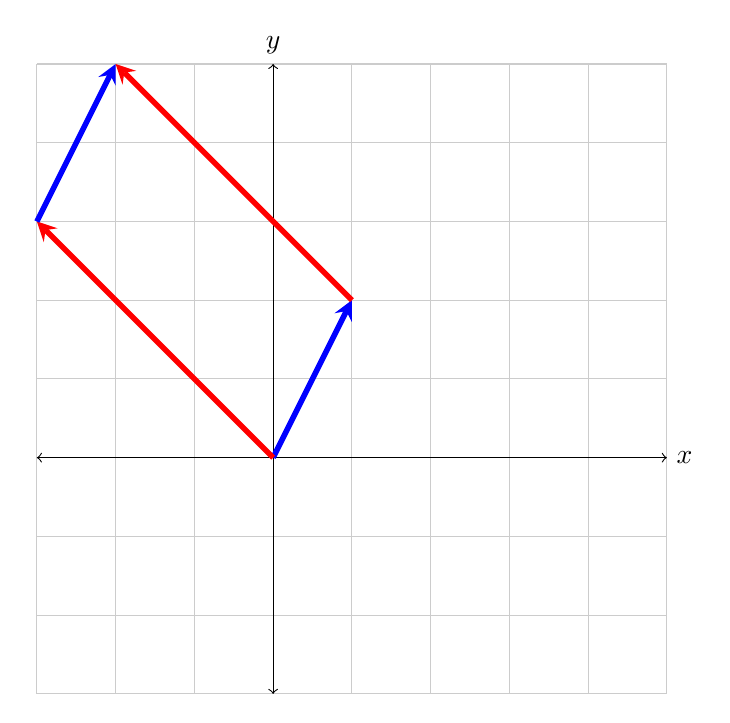
\begin{tikzpicture}
        \draw[thin,gray!40] (-3,-3) grid (5,5);
        \draw[<->] (-3,0)--(5,0) node[right]{$x$};
        \draw[<->] (0,-3)--(0,5) node[above]{$y$};
        \draw[line width=2pt,blue,-stealth](0,0)--(1,2) node[anchor=west] at (1,2){$\vecu$};
        \draw[line width=2pt, red, -stealth](0,0)--(-3,3) node[anchor=north] at (-3,3){$\vecv$};
        \draw[line width=2pt, blue, -stealth](-3,3)--(-2,5) node[anchor=west] at (-2,5){};
        \draw[line width=2pt, red, -stealth](1,2)--(-2,5) node[anchor=west] at (-2,5){};
        \end{tikzpicture}
        \end{center}
        In order to compute this area, we can use the cross product by thinking of these vectors as being in $3$-dimensional space by
        \[
        \vecu = 1\xhat + 2\yhat + 0\zhat \qquad \textrm{and} \qquad \vecv = -3\xhat +3\yhat + 0\zhat.
        \]
        Then the cross product of these two vectors must only have a $z$-component since these two vectors lie in the $xy-$plane. Thus, we can compute
        \begin{align*}
            \vecu \times \vecv = (1\cdot 3 - (-3)\cdot2)\zhat = 9\zhat.
        \end{align*}
        Hence, the area is $\|\vecu\times \vecv\| = \|9\zhat \| = 9.$
\end{enumerate}
\end{solution}

\newpage
\begin{problem}~
\begin{enumerate}[(a)]
    \item We can reflect a vector in the plane by first reflecting basis vectors. Let $R\colon \R^2 \to \R^2$ be a function be defined by 
    \[
    R(\xhat) = -\xhat \qquad \textrm{and} \qquad R(\yhat)=\yhat.
    \]
    Let $\vecv = \alpha_1 \xhat + \alpha_2 \yhat$ and define
    \[
    R(\vecv) = \alpha_1 R(\xhat) + \alpha_2 R(\yhat).
    \]
    When this is the case, we call the function $T$ \underline{linear}.\\
    \noindent Show that $R$ reflects the vector $\vecu = 1\xhat + 2\yhat$ about the $y$-axis and draw a picture.
    \item We can rotate a vector in the plane by first rotating the basis vectors $\xhat$ and $\yhat$. Define a \underline{linear} function $T\colon \R^2 \to \R^2$ defined by
    \[
    T(\xhat)=\yhat \qquad \textrm{and} \qquad T(\yhat)=-\xhat.
    \]
    \noindent Show that $T$ rotates $\vecu$ by $\pi/2$ in the counterclockwise direction and draw a picture.
\end{enumerate}
\end{problem}
\begin{solution}~
\begin{enumerate}[(a)]
    \item So, we can take the vector $\vecu$ and then we have
    \[
    R(\vecu)=1R(\xhat)+2R(\yhat) = -1\xhat +2\yhat.
    \]
    So we can plot both $\vecu$ and $R(\vecu)$ in the plane:
        \begin{center}
        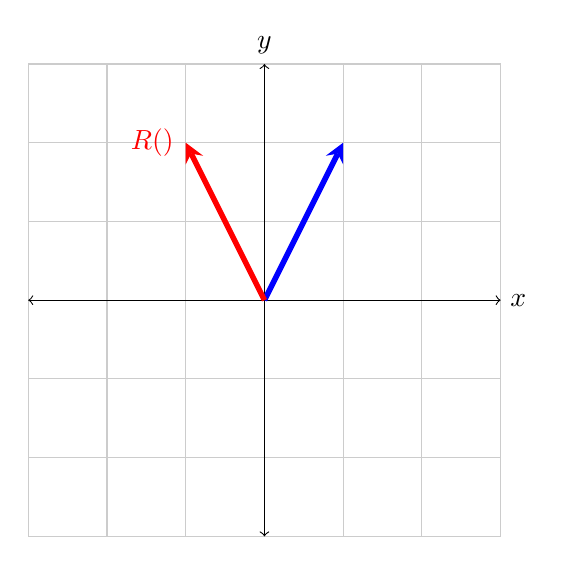
\begin{tikzpicture}
        \draw[thin,gray!40] (-3,-3) grid (3,3);
        \draw[<->] (-3,0)--(3,0) node[right]{$x$};
        \draw[<->] (0,-3)--(0,3) node[above]{$y$};
        \draw[line width=2pt,blue,-stealth](0,0)--(1,2) node[anchor=west] at (1,2){$\vecu$};
        \draw[line width=2pt, red, -stealth](0,0)--(-1,2) node[anchor=east] at (-1,2){$R(\vecu)$};
        \end{tikzpicture}
        \end{center}
        We can see that this is definitely the reflection of the vector $\vecu$ across the $y$-axis.
    \item We can now do this for the function $T$ to get
    \[
    T(\vecu) = 1T(\xhat)+2T(\yhat)=1\yhat -2\xhat.
    \]
    Then we can plot both $\vecu$ and $T(\vecu)$ in the plane:
        \begin{center}
        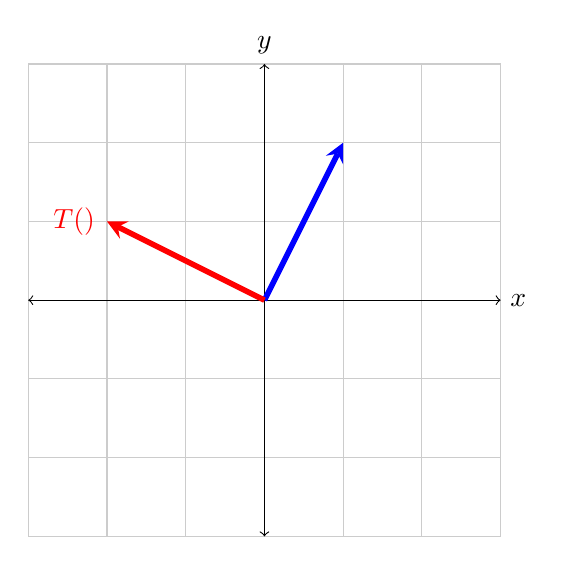
\begin{tikzpicture}
        \draw[thin,gray!40] (-3,-3) grid (3,3);
        \draw[<->] (-3,0)--(3,0) node[right]{$x$};
        \draw[<->] (0,-3)--(0,3) node[above]{$y$};
        \draw[line width=2pt,blue,-stealth](0,0)--(1,2) node[anchor=west] at (1,2){$\vecu$};
        \draw[line width=2pt, red, -stealth](0,0)--(-2,1) node[anchor=east] at (-2,1){$T(\vecu)$};
        \end{tikzpicture}
        \end{center}
        We can see that this is definitely the rotation  of the vector $\vecu$ an angle of $\pi/2$ in the counter-clockwise direction.
\end{enumerate}
\end{solution}

\newpage
\begin{problem}
Consider the following vectors in space $\R^3$
\[
\vecu = 1\xhat + 2\yhat + 3\zhat \qquad \textrm{and} \qquad \vecv = -2\xhat +1\yhat -2\zhat.
\]
\begin{enumerate}[(a)]
    \item Compute the dot product $\vecu\cdot \vecv$. 
    \item Compute the cross product $\vecu \times \vecv$.
    \item \textbf{(Experimental)} Let us try this: Take
    \begin{align*}
        \vecu \vecv &= (1\xhat + 2\yhat + 3\zhat)(-2\xhat + 1\yhat -2\zhat).
    \end{align*}
    Distribute the above multiplication.
    \item \textbf{(Experimental)} Now, in the above multiplication, adopt the following rules:
    \begin{align*}
        \xhat \xhat = \yhat \yhat = \zhat \zhat &= 1 &&&
        \xhat \yhat &= - \yhat \xhat &&& \xhat \zhat &= - \zhat \xhat &&& \yhat \zhat &= -\zhat \yhat.
    \end{align*}
    Then, simplify the multiplication in part (c) to
    \[
    \vecu\vecv = \alpha + \beta_1 \yhat\zhat  \ + \beta_2 \zhat \xhat + \beta_3 \xhat \yhat. 
    \]
    That is, what are $\alpha$, $\beta_1$, $\beta_2$, and $\beta_3$?
    \item \textbf{(Experimental)} If we perform one more step, we will notice something quite nice.  Note that the pairs of vectors above define a plane, and there is a unique vector perpendicular to that plane.  Using this fact, we can let 
    \[
    \yhat \zhat = \xhat \qquad \zhat \xhat = \yhat \qquad \xhat \yhat = \zhat.
    \]
    In other words, we can replace the two vectors above with their cross product, (i.e., $\yhat \zhat = \yhat \times \zhat = \xhat$.) Show that with these rules
    \[
    \vecu \vecv = \vecu\cdot \vecv + \vecu \times \vecv.
    \]
\end{enumerate}
\end{problem}
\begin{solution}~
\begin{enumerate}[(a)]
    \item We have that
    \begin{align*}
        \vecu \cdot \vecv &= 1\cdot (-2) + 2 \cdot 1 + 3 \cdot (-3)\\
        &= -6.
    \end{align*}
    \item Here, feel free to use a formula for a cross product instead of writing it all out.  We will find that
    \begin{align*}
        \vecu \times \vecv &= -7\xhat -4\yhat +5\zhat.
    \end{align*}
    \item Note, I put experimental in these following parts as they are \underline{not} the traditional way of teaching these topics. However, I think this methodogology gives a more intuitive notion of vectors than the traditional dot and cross products.
    
    So we have
    \begin{align*}
        \vecu \vecv &= (1\xhat + 2\yhat +3\zhat)(-2\xhat +1\yhat -2\zhat)\\
        &= -2\xhat\xhat + 1 \xhat \yhat - 2\xhat \zhat \\
        &~ + -4\yhat \xhat + 2\yhat \yhat -4\yhat \zhat \\
        &~ + -6\zhat \xhat +3\zhat \yhat -6\zhat \zhat.
    \end{align*}
    \item Now, we can use the rules to find that we get
    \begin{align*}
        \vecu\vecv &= (-2 +2 - 6) + (-4-3)\yhat \zhat + (-6+2)\zhat \xhat + (1+4)\xhat \yhat\\
        &= -6  -7 \yhat \zhat - 4\zhat \xhat +5 \xhat \yhat.
    \end{align*}
    Hence, we have $\alpha = -6$, $\beta_1 = -7$, $\beta_2=-4$, $\beta_3 = 5$.
    
    Here we can imagine that there are units attached to the quantities $\xhat$, $\yhat$, and $\zhat$.  There is a scalar quantity which contains none of these unit vectors, and there are quantities which contain two (i.e., $\xhat\yhat$).  The quantities containing two unit vectors represent the plane given by the two vectors.
    \item Now, we can identify a unit vector perpendicular to a plane in $\R^3$ that satisfies the right hand rule given by the cross product.  In which case, we replace the above ``multivectors" (i.e., $\xhat\yhat$) with the unique unit vector perpendicular to the two.  So we have
    \[
    \vecu \vecv = -6 -7\xhat -4\yhat +5\zhat,
    \]
    which is indeed giving us that
    \[
    \vecu \vecv = \vecu\cdot \vecv + \vecu \times \vecv.
    \]
\end{enumerate}

\begin{remark}
This all falls under the mathematics of \emph{geometric algebra} which is a more general way of understanding vectors.  It is rather useful, yet it is not quite mainstream.  Maybe one day it will be!
\end{remark}

\end{solution}

\newpage
\begin{problem}
Consider the same vectors $\vecu,\vecv\in \R^3$ from Problem 4.  
\begin{enumerate}[(a)]
    \item Compute the lengths $\|\vecu\|$ and $\|\vecv\|$ using the dot product.
    \item Compute the angle between vectors $\vecu$ and $\vecv$. \emph{Hint: Save some work and use results from Problem 4.}
    \item Compute the projection of $\vecu$ in the direction of $\vecv$. \emph{Hint: Again, save yourself some time and use results from Problem 4.}
\end{enumerate}
\end{problem}
\begin{solution}~
\begin{enumerate}[(a)]
    \item Note that we have
    \[
    \|\vecu \| = \sqrt{ \vecu \cdot \vecu}
    \]
    and so we have
    \[
    \|\vecu \| = \sqrt{1^2+2^2+3^2} = \sqrt{14}.
    \]
    Similarly,
    \[
    \|\vecv\| = \sqrt{(-2)^2+1^2+(-2)^2} = \sqrt{9}=3.
    \]
    \item Now, we found $\vecu\cdot \vecv = -6$ and we have
    \[
    \vecu \cdot \vecv = \|\vecu\|\|\vecv \| \cos \theta
    \]
    as well. Hence, it follows that
    \begin{align*}
        \theta &= \arccos\left(\frac{\vecu \cdot \vecv}{\|\vecu\|\|\vecv\|}\right)\\
        &= \arccos\left(\frac{-6}{\sqrt{14}\cdot 3}\right)\\
        &\approx  2.1347 \approx 122.3^\circ.
    \end{align*}
    \item To compute this projection of $\vecu$ onto the direction of $\vecv$, we must first normalize $\vecv$ to make $\boldsymbol{\hat{v}}$. We have
    \[
    \boldsymbol{\hat{v}} = \frac{\vecv}{\|\vecv\|} = -\frac{2}{3}\xhat + \frac{1}{3}\yhat - \frac{2}{3}\zhat.
    \]
    Then we can compute the projection by
    \begin{align*}
        (\vecu \cdot \boldsymbol{\hat{v}})\boldsymbol{\hat{v}}&= \left((\xhat + 2\yhat + 3\zhat ) \cdot \left( -\frac{2}{3}\xhat + \frac{1}{3}\yhat - \frac{2}{3}\zhat\right)\right) \boldsymbol{\hat{v}} \\
        &= 2\boldsymbol{\hat{v}}.
    \end{align*}
    You could also just compute
    \[
    \frac{\vecu \cdot \vecv}{\|\vecv\|^2}\vecv
    \]
    and get the same answer.
\end{enumerate}
\end{solution}
\end{document}